\documentclass[letter, 10pt]{article}
\usepackage[utf8]{inputenc}
\usepackage{enumerate}
\usepackage[spanish]{babel}
\usepackage{amsfonts}
\usepackage{amsmath}
\usepackage{nomencl}
\usepackage{url}
\usepackage{eucal}
\usepackage[pdftex]{graphicx}
\usepackage{float}
\usepackage{listings}
\usepackage[ruled,vlined,linesnumbered]{algorithm2e}
\usepackage[top=3cm,bottom=3cm,left=3.5cm,right=3.5cm,footskip=1.5cm,headheight=1.5cm,headsep=.5cm,textheight=3cm]{geometry}



\begin{document}
\title{Inteligencia Artificial \\ \begin{Large}Informe Final: Vehicle Routing Problem with Backhouls (VRPB)\end{Large}}
\author{Francisco Abarca Moraga\\201673552-6}
\date{\today}
\maketitle


%--------------------No borrar esta secci\'on--------------------------------%
\section*{Evaluaci\'on}

\begin{tabular}{ll}
Mejoras 1ra Entrega (10\%): &  \underline{\hspace{2cm}}\\
C\'odigo Fuente (10\%): &  \underline{\hspace{2cm}}\\
Representaci\'on (15\%):  & \underline{\hspace{2cm}} \\
Descripci\'on del algoritmo (20\%):  & \underline{\hspace{2cm}} \\
Experimentos (10\%):  & \underline{\hspace{2cm}} \\
Resultados (10\%):  & \underline{\hspace{2cm}} \\
Conclusiones (20\%): &  \underline{\hspace{2cm}}\\
Bibliograf\'ia (5\%): & \underline{\hspace{2cm}}\\
 &  \\
\textbf{Nota Final (100)}:   & \underline{\hspace{2cm}}
\end{tabular}
%---------------------------------------------------------------------------%
\vspace{2cm}


\begin{abstract}
El VRPB es el problema que modela una flota de vehículos, los cuales deben entregar y recolectar productos a determinados clientes los cuales están dispersos geográficamente, además, los vehículos de la flota tienen una capacidad determinada para los productos. Estos vehículos deben realizar las entregas antes de realizar cualquier recolección, además deben volver al punto desde el cual inició su trayecto el cual se denomina como depósito. La finalidad es encontrar las rutas óptimas en donde todos los clientes son visitados y se minimiza la distancia recorrida por la flota. Como primer objetivo en este documento se ahonda en el contenido del problema para conocerlo de mejor manera. Para esto, se revisa qué métodos han sido utilizados para resolverlo, mediante la investigación del estado del arte. El segundo objetivo es exponer los resultados obtenidos al resolver una instancia del problema con una técnica de búsqueda completa, Forward Checking and Graph-Based backjumping.
\end{abstract}

\section{Introducción}

Los problemas de ruteo de vehículos o VRP, son problemas de optimización, los cuales buscan diseñar rutas en donde se trata de minimizar los costos, dada una flota de vehículos hospedada en un depósito o centro de distribución, que proporcionan un servicio a un conjunto de clientes, los cuales se encuentran dispersos geográficamente. Dado el costo que atrae una red de distribución física se genera esta variante del VRP, el Vehicle Routing Problem with Backhauls (VRPB). Esta variante, se aprovecha los vehículos que hacen entregas de productos, para ser usados en recibir productos hacia el depósito en su viaje de regreso. Esto implica considerar la capacidad de la flota para el proceso de recepción de productos, como también que cada ruta complete todas las entregas antes de realizar recepciones y que estas no violen la capacidad de carga de los vehículos. El objetivo es buscar un conjunto de rutas el cual minimice el total de distancia recorrida por la flota.
\\\par
Con la finalidad de explorar los datos obtenidos al realizar una búsqueda completa para el VRPB, en este documento se iniciará con una definición del problema, esto consiste en primera instancia de una explicación del problema y lo necesario que es usado para su modelo matemático. Luego, una presentación del estado del arte, que incluye las perspectivas que han sido utilizadas para atacar el problema. A continuación, se formula el modelo matemático del problema, incluyendo la función objetivo en conjunto con las restricciones. Después, se describe la representación de las soluciones, en esta sección se describe como serán tratadas. De modo siguiente se presenta una descripción del algoritmo utilizado y como se experimentó con el. Y a modo de cierre, se expondrán los resultados y las conclusiones del estudio elaborado.

\section{Definición del Problema}
El rápido crecimiento de los mercados, a generado un problema a nivel de distribución logística de los productos. Se ha reportado que los costes de logística en los productos abarcan un 22.5\%, esto sobre el costo de manufactura de los productos \cite{kearney1984measuring}, por lo tanto, es necesario reducir estos costos para obtener una ventaja competitiva dentro de los mercados. Una forma de mejorar esta situación es usar las redes que hacen entregas y reutilizarlas para recoger productos antes de volver a los depósitos. Sin embargo, estamos limitados a rutas factibles luego de entregar los productos iniciales por los vehículos de la red logística. Esta situación se modela utilizando los siguientes componentes: Un conjunto de clientes esperando entregas, un conjunto de clientes esperando enviar productos, ambos conjuntos distribuidos geográficamente; un depósito, el cual tiene disponible la flota de vehículos, estos con una capacidad determinada, los cuales deben visitar a los clientes y satisfacer sus demandas.
\\\par
VRPB consiste en determinar las rutas para los vehículos, estas rutas empiezan y terminan en el mismo depósito, donde cada cliente debe ser visitado exactamente una vez y cada vehículo viaja solo una ruta, una ruta puede estar compuesta solamente por entregas, pero no por despachos. Para que un vehículo acepte despachos, este debe haber realizado todas sus entregas, así como la suma de los productos de entrega y despacho, por separado, no pueden exceder la capacidad del vehículo. Una dificultad que se asoma, es el identificar casos de no conectividad entre los nodos, o cuando, esto genera subproblemas a resolver dentro del problema principal. Otro punto a considerar, es la naturaleza del problema, al ser un problema derivado de VRP este es NP-Hard, por lo tanto, la obtención de una solución exacta para una instancia se vuelve complejo, a medida que crece el problema, de forma exponencial \cite{lenstra1981complexity}.


\subsection{Variantes del Problema}
Existen diversas extensiones de VRPB, de las cuales la más cercana es Mixed Vehicle Routing Problem with Backhauls o MVRPB \cite{wade2002investigation}, en donde la restricción de concretar las entregas, antes de realizar despachos es eliminada. Por otra parte, se encuentra Multi-Depot Vehicle Routing Problem (MDVRP)\cite{crevier2007multi}, al cual también se le ha agregado la variante con despachos MDVRPB, este problema añade complejidad al aumentar la cantidad de depósitos disponibles, esto a su vez aumenta la cantidad de decisiones a tomar, ya no es solo generar las rutas, sino asignar los vehículos a los clientes disponibles según la distribución geográfica de los clientes, esto en relación con los depósitos disponibles.

Además cabe notar el problema VRP with Pick-ups and Deliveries (VRPPD)\cite{desaulniers2002vrp}, este problema contiene el estudiado, esto quiere decir que VRPB es una variante de VRPPD, la idea de VRPPD es que existen solicitudes de transporte que deben ser satisfechas, estas consisten en un punto de entrega y otro de despacho, para satisfacer el problema, deben encontrarse rutas que reciban los paquetes y sean enviados a sus destinos, similar a MVRPB.

\section{Estado del Arte}
La familia de problemas VRP fue introducida el año 1959, por Dantzig y Ramser \cite{bernard1959truck}, la finalidad era sobre el envío de petróleo por una flota de vehículos, el incentivo era disminuir los precios del sector al minimizar costos de transporte, aún más relevante considerando que el 10\% del GDP de la unión europea, esta sostenido por la industria del transporte\cite{hasle2007geometric}. La variante estudiada (VRPB), data a mediados de los 80 \cite{golden1985vehicle}. A continuación, se presentan distintas metodologías utilizadas para resolver el VRPB:
\subsection{Acercamiento inicial}
Dadas las restricciones adicionales que incluye el VRPB de un VRP, sea el hecho de incluir despachos en las rutas, las métricas o heurísticas utilizadas deben ser modificadas para el problema en cuestión. En una primera instancia se determinó, que el uso de heurísticas era lo más óptimo para resolver problema \cite{goetschalckx1989vehicle}.

La eficiencia en la solución se daría en dos pasos, primero, usar algoritmos de naturaleza polinomial y segundo, encontrar una buena solución inicial, esto dado que existe una gran chance de terminar cerca de una solución óptima, al utilizar una heurística. En la época se hizo uso de Space Filling Curves (SFC), este método mantiene el sentido de cercanía entre los puntos, además de ser rápidas, la calidad de la solución inicial obtenida es alta \cite{bartholdi1988heuristics}.

Con la solución inicial se aplican heurísticas, la más notable es la K-mediana, esta implica dado n puntos, elegir K puntos como "medianas" de tal forma que la distancia entre cada punto a su mediana más cercana sea mínimo. Esto cumple con la primera fase, dado que el algoritmo tiene un esfuerzo computacional de $O(n \log n)$ y un peor caso de $2\sqrt{n}$.

El algoritmo generado es el siguiente:

\begin{enumerate}
    \item Transformar el conjunto de puntos de entrega mediante la heurística SFC, formando una lista ordenada de puntos a un intervalo fijo.
    \item Agrupar los puntos
    \item Enrutar los puntos visitando los puntos en cada agrupación, en el orden que aparecen en la lista ordenada, forma ascendente.
    \item Repetir pasos (1)-(3) con los puntos de despacho.
    \item Enlazar cada ruta de entrega a su correspondiente ruta de despacho y al centro de distribución.
\end{enumerate}

El agrupamiento de los puntos es realizado vía un algoritmo greedy, cabe mencionar que el problema de las K-medianas omite la restricción de capacidad, por lo tanto es posible encontrar agrupaciones de puntos que sobrepasen la capacidad en ciertas rutas. En general este método sacrifica calidad de solución por tiempo de ejecución, en valores numéricos de la época, el algoritmo es 4 veces más rápido en una instancia de 110 clientes que el método de Clark y Wright \cite{clarke1964scheduling} ampliamente utilizado en la usos comerciales a esa fecha, con una penalización de solución cercana al 15\%.

\subsection{Algoritmo genéticos}
Algoritmos evolutivos son una amplia clase dentro de las meta-heurísticas, estas son inspiradas mediante metáforas dadas en la naturaleza, donde los algoritmos genéticos (GA)\cite{goldberg1989genetic} corresponden a uno de los más conocidos. Básicamente, imitan la forma en que las especies evolucionan y se adaptan a su entorno, según el principio Darwiniano de la selección natural.

Bajo este paradigma, una población de soluciones (usualmente codificada como bits o cadenas de caracteres, conocidas como cromosomas) evoluciona de una generación a la próxima, mediante el uso de operadores encontrados en la naturaleza, sea la selección de los individuos (cromosomas) más aptos, recombinaciones y mutaciones. Con el uso de estos operadores, sólo las mejores soluciones son permitidas a ser padres de las generaciones siguientes. El proceso de entrecruzamiento o recombinación, toma dos soluciones padres y combina las características más deseables para generar uno o más hijos. Esto es repetido hasta que se ha obtenido una nueva población. Finalmente, cada elemento de la nueva población es perturbado aleatoriamente por un operador de mutación. Empezando por una población inicial generada mediante heurísticas o aleatoriedad, el ciclo anterior es repetido una cantidad de generaciones, y la mejor solución encontrada es retornada al final.

El esquema GA es modificado al ser utilizado en problemas de la familia VRP. En particular, la codificación de las soluciones es ignorada o diseñada en una forma particular para tomar ventaja del entrecruzamiento especializado y operadores de mutación.

Estudios \cite{potvin1996genetic} con esta heurística muestran soluciones que fluctúan cercano al 1\% del óptimo en promedio, en modelos de hasta 200 clientes. La dificultad de este algoritmo es encontrar una solución factible inicial, para el inicio de las búsquedas locales.

\subsection{Búsqueda tabú}
Búsqueda tabú \cite{glover1997tabu} es una meta-heurística basada en búsqueda local donde, en cada iteración, la mejor solución en la comunidad de la solución actual es seleccionada como la nueva solución actual, incluso si incrementa el costo de la solución. Mediante este mecanismo, el método puede escapar de un óptimo local no beneficioso. Una memoria a corto plazo, llamada lista tabú, almacena soluciones recientemente visitadas (o atributos de soluciones visitadas recientemente) para evitar ciclos cortos. Esto es realizado cada vez dada una modificación que lidera a una nueva solución, la modificación inversa es listada como tabú y es guardada en la lista. La búsqueda para dado una cantidad fija de iteraciones, o luego de iterar sin mejorar la solución superior conocida de forma consecutiva.

Un estudio inicial \cite{duhamel1997tabu} demostró la capacidad del uso de esta meta-heurística, superando al algoritmo GA con un 0.5\% sobre el óptimo en promedio, además de tener un menor impacto computacional. Un estudio más actual \cite{brandao2006new}, indaga en nuevos métodos como la integración de pseudo-límites, el uso de distintas formulaciones del algoritmo de TSA (Tabu search algorithm) y el uso de una mayor cantidad de soluciones iniciales.

\subsection{Algoritmos exactos}
Inicialmente se buscaron algoritmos para buscar soluciones exactas para el VRPB, luego de propuestas dos variantes \cite{mingozzi1999exact}\cite{toth1997exact} (ambas consideran relajación lagrangiana, la cual penaliza las restricciones según su importancia generando una solución aproximada al problema general, y set partitioning), el problema de investigar algoritmos exactos no era factible. Esto debido mayormente a la complejidad del problema, por lo tanto, es recomendado el uso de métodos que empleen heurísticas para problemas con más de 110 clientes.

Eso indicaba la literatura hace poco, un nuevo artículo \cite{queiroga2020exact}, al hacer uso de algoritmos tipo Branch-Cut-and-Price (BCP) e integrarlos a las propuestas anteriores. Los nuevos algoritmos mejorados, son capaces de resolver instancias de hasta 200 clientes sin mayor complejidad con un tiempo menor a los 100 segundos de ejecución y al menos 25\% de los conjuntos fueron resueltos a optimalidad.

\section{Modelo Matemático}
Para la formulación matemática del VRPB se utiliza como referencia el trabajo de Paolo Toth y Daniele Vigo \cite{toth2002vehicle}. El problema puede ser representado mediante el siguiente modelo de teoría de grafos, donde cada cliente corresponde a un vértice.

Sea $G = (V, A)$ un grafo no dirigido completo, con un conjunto de vértices $V := \{0\} \cup L \cup B$. Subconjuntos $L = \{1,\dots,n\}$ y $B = \{n+1,\dots,n+m\}$ corresponden a los conjuntos de clientes de entregas (Linehaul) y despachos (Backhauls) respectivamente. Una cantidad positiva, $d_j$, de producto es entregada o recogida (demanda), la cual es asociada con cada vértice $j \in V \setminus \{0\}$. El vértice $0$ corresponde al depósito (con una demanda ficticia de $d_0=0$), donde $K$ vehículos idénticos con una capacidad dada de $C$, se encuentran estacionados. Sea $c_{ij}$ el costo (valor no negativo) asociado con el arco $(i,j) \in A$, con $c_{ii} = +\infty$ para cada $i \in V$ (y con $c_{ij} = c_{ji}$ para cada $i, j \in V$ cuando $i \neq j$).

El modelo además define ciertas notaciones adicionales, $L_0 := L \cup \{0\}$ y $B_0 := B \cup \{0\}$, como los nuevos conjuntos para las entregas y despachos, los cuales incluyen el depósito. Además sea $\overline{G}=(\overline{V}, \overline{A})$, un grafo dirigido obtenido al definir $\overline{V} = V$ y $\overline{A} = A_1 \cup A_2 \cup A_3$, donde:

$$A_1 := \{(i, j) \in A : i \in L_0, j \in L\},$$
$$A_2 := \{(i, j) \in A : i \in B, j \in B_0\},$$
$$A_3 := \{(i, j) \in A : i \in L, j \in B_0\}.$$

Estos tres subconjuntos representan:
\begin{enumerate}
    \item Todos los arcos desde el depósito y entregas hacia vértices de entregas
    \item Todos los arcos desde despachos hacia vértices de despachos y el depósito
    \item Todos los arcos que conectan vértices de entregas hacia despachos y el depósito
\end{enumerate}

Notar que el conjunto $\overline{A}$, no contiene arcos que no contribuyen a la solución, estos son filtrados mediantes los subconjuntos definidos anteriormente, además, los valores $c_{ij}$ asociados a los arcos son iguales a los considerados en el conjunto $A$.

Además se debe declarar, $\CMcal{L}$ (análogo para $\CMcal{B}$) como la familia de todos los subconjuntos de vértices en $L$ (análogo para $B$), y $\CMcal{F} = \CMcal{L} \cup \CMcal{B}$. Para cada $\CMcal{S} \in \CMcal{F}$, se calcula $r(\CMcal{S})$ como el mínimo número de vehículos necesitado para servir a todos los clientes en $\CMcal{S}$. Este valor es calculado como el valor óptimo del Bin Packing Problem (BPP), con un conjunto de $\CMcal{S}$ elementos con una capacidad de $C$. Finalmente, denotamos para cada $i \in V$ lo siguiente, $\Delta_i^+ = \{j : (i, j) \in \overline{A}\}$ (estrella creciente de i) y $\Delta_i^- = \{j : (j, i) \in \overline{A}\}$ (estrella decreciente de i).

El modelo matemático resultante es el siguiente:

\subsection*{Consideraciones del problema}
\begin{enumerate}[(i)]
  \item Cada vehículo es usado a lo más en una ruta
  \item Cada circuito visita el vértice $0$, tanto al inicio como al final de la ruta
  \item Cada vértice $j \in V \setminus \{0\}$ es visitado únicamente
  \item La suma de las demandas de entrega y despacho visitadas en una ruta no exceden, separadamente, la capacidad $C$
  \item En cada circuito las entregas preceden a los despachos, en caso de haber alguno
\end{enumerate}

\subsection*{Parámetros}
\begin{itemize}
    \item $K$: Cantidad de vehículos en la flota
    \item $C$: Capacidad de carga de cada vehículo en la flota
    \item $n$: Cantidad de clientes que requieren entregas
    \item $m$: Cantidad de clientes que requieren despachos
    \item $c_{ij}$: Costo de viajar desde el nodo $i$ al nodo $j$
    \item $d_i$: Demanda de capacidad del cliente $i$
    \item $r(\CMcal{S})$: Valor óptimo del BPP para el conjunto $\CMcal{S}$ con capacidad $C$, el cual tiene un límite inferior de $\lceil d(\CMcal{S})/C \rceil$
\end{itemize}

\subsection*{Variables}
\begin{itemize}
    \item $x_{ij}$: Variable binaria, 1 si se viaja desde $i$ hacia $j$, 0 en caso contrario $\forall (i, j) \in \overline{A}$
\end{itemize}

\subsection*{Función Objetivo}
Minimizar la distancia total recorrida por la flota de vehículos
$$ min \sum_{(i, j) \in \overline{A}} c_{ij} x_{ij} $$

\subsection*{Restricciones}

\begin{equation} 
 \sum_{i \in \Delta_j^-} x_{ij} = 1 \qquad \forall j \in \overline{V} \in \setminus \{0\}
\end{equation}
\begin{equation} 
 \sum_{j \in \Delta_i^+} x_{ij} = 1 \qquad \forall i \in \overline{V} \in \setminus \{0\}
\end{equation}
\begin{equation} 
 \sum_{i \in \Delta_0} x_{i0} = K
\end{equation}
\begin{equation} 
 \sum_{j \in \Delta_0^+} x_{0j} = K
\end{equation}
\begin{equation} 
 \sum_{j \in \CMcal{S}} \sum_{i \in \Delta_j^- \setminus \CMcal{S}} x_{ij} \geq \lceil \sum_{j \in \CMcal{S}} d_j / D \rceil \qquad \forall \CMcal{S} \in \CMcal{L}
\end{equation}
\begin{equation} 
 \sum_{i \in \CMcal{S}} \sum_{j \in \Delta_i^+ \setminus \CMcal{S}} x_{ij} \geq \lceil \sum_{j \in \CMcal{S}} d_j / D \rceil \qquad \forall \CMcal{S} \in \CMcal{B}
\end{equation}

Las restricciones (1)-(4) imponen que los nodos deben ser visitados una solo vez, además de asegurarse que todos sean visitados, y las restricciones (5)-(6) verifican que la capacidad de carga de las rutas no sobrepase a los vehículos asignados.

\subsection*{Naturaleza de las variables}
$$ x_{ij} \in \{0, 1\}, \qquad \forall (i, j) \in \overline{A}$$

\subsection*{Representación gráfica de una instancia}
Se muestra a continuación una solución a una instancia, de manera visual se aprecia como se separan los conjuntos y la nomenclatura utilizada dentro del problema.
\newline

\begin{center}
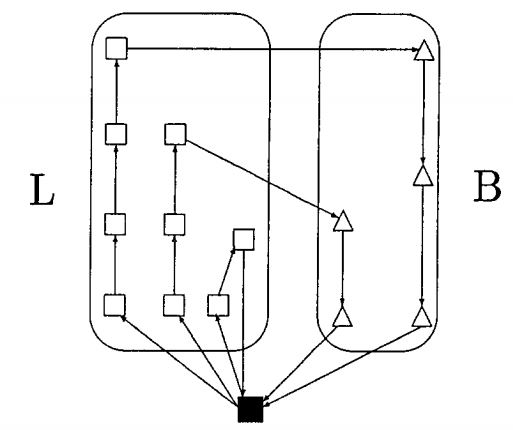
\includegraphics[scale=0.5]{Red.PNG}
\end{center}

\section{Representación}
Para la representación del problema se utilizó el sistema de variables binario $x_{ijk}$ utilizado por Goestchalckx et al. (1989) \cite{goetschalckx1989vehicle}, donde la variable indica si se viaja desde el cliente $i$ hacia el $j$ mediante la ruta/vehículo $k$. El dominio de esta variable corresponde a los valores $0$ o $1$ dada la naturaleza binaria mencionada anteriormente.

\begin{center}
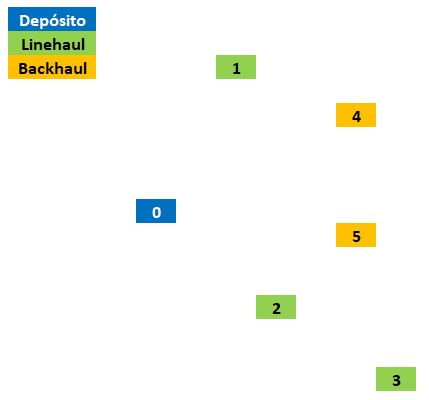
\includegraphics[scale=0.5]{Instancia inicial.jpg}
\end{center}

Como ejemplo la imagen superior representa una disposición de $6$ clientes (1 depósito, 3 linehauls, 2 backhauls), para la cual se disponen de 2 rutas. Este ejemplo supone la siguiente representación:

\[ 
\left(
\begin{matrix}
 x_{000} &  x_{010} &  x_{020} &  x_{030} &  x_{040} &  x_{050}\\ 
 x_{100} &  x_{110} &  x_{120} &  x_{130} &  x_{140} &  x_{150}\\ 
 x_{200} &  x_{210} &  x_{220} &  x_{230} &  x_{240} &  x_{250}\\ 
 x_{300} &  x_{310} &  x_{320} &  x_{330} &  x_{340} &  x_{350}\\ 
 x_{400} &  x_{410} &  x_{420} &  x_{430} &  x_{440} &  x_{450}\\ 
 x_{500} &  x_{510} &  x_{520} &  x_{530} &  x_{540} &  x_{550}
\end{matrix}
\right)
%
\left(
\begin{matrix}
 x_{001} &  x_{011} &  x_{021} &  x_{031} &  x_{041} &  x_{051}\\ 
 x_{101} &  x_{111} &  x_{121} &  x_{131} &  x_{141} &  x_{151}\\ 
 x_{201} &  x_{211} &  x_{221} &  x_{231} &  x_{241} &  x_{251}\\ 
 x_{301} &  x_{311} &  x_{321} &  x_{331} &  x_{341} &  x_{351}\\ 
 x_{401} &  x_{411} &  x_{421} &  x_{431} &  x_{441} &  x_{451}\\ 
 x_{501} &  x_{511} &  x_{521} &  x_{531} &  x_{541} &  x_{551}
\end{matrix}
\right)
\]

Una solución visual del problema correspondería a desplegar dos rutas que cubran a todos los clientes, siguiendo el orden de linehauls y luego backhauls de forma excluyente. La siguiente imagen representa una solución (sin considerar la capacidad de las rutas, ni las demandas de los clientes), la cual explicita las dos rutas utilizadas (la primera ruta que corresponde a $ 0 \rightarrow 1 \rightarrow 4 \rightarrow 0 $. La segunda ruta de color azul, corresponde a $0 \rightarrow 2 \rightarrow 3 \rightarrow 5 \rightarrow 0$).

\begin{center}
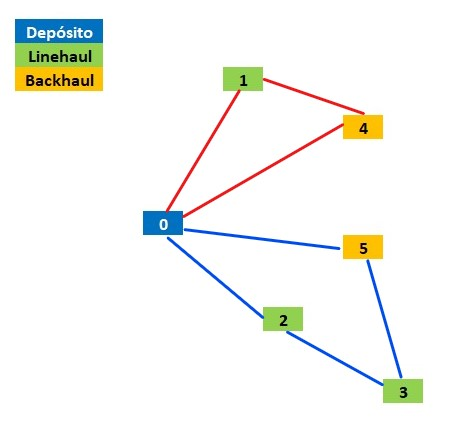
\includegraphics[scale=0.5]{Instancia final.jpg}
\end{center}

La instanciación de la solución mediante la representación con variables es la siguiente:

\[ 
\left(
\begin{matrix}
0 & 1 & 0 & 0 & 0 & 0\\
0 & 0 & 0 & 0 & 1 & 0\\
0 & 0 & 0 & 0 & 0 & 0\\
0 & 0 & 0 & 0 & 0 & 0\\
1 & 0 & 0 & 0 & 0 & 0\\
0 & 0 & 0 & 0 & 0 & 0
\end{matrix}
\right)
%
\left(
\begin{matrix}
0 & 0 & 1 & 0 & 0 & 0\\
0 & 0 & 0 & 0 & 0 & 0\\
0 & 0 & 0 & 1 & 0 & 0\\
0 & 0 & 0 & 0 & 0 & 1\\
0 & 0 & 0 & 0 & 0 & 0\\
1 & 0 & 0 & 0 & 0 & 0
\end{matrix}
\right)
\]

Cabe notar que no es posible utilizar la representación triangular de las matrices, dado que las matrices no son simétricas, esto es efecto de la naturaleza dirigida de las rutas. Existen diversas formas de representar las rutas, algunas encapsulan la dimensión de las rutas al cambiar el dominio de la variable a que ruta corresponde la variable, esto a cambio de generar mayor complejidad del programa.

\section{Descripción del algoritmo}
El algoritmo utilizado corresponde a Forward Checking (FC) con Backjumping basado en restricciones (GBJ). El algoritmo es de naturaleza completa, esto se refiere a que itera sobre todo el dominio de búsqueda e intenta encontrar todas las soluciones posibles del problema. Dada la naturaleza combinatoria del problema, el dominio crece muy rápido a medida que aumentan los clientes y rutas a utilizar (A una cifra de $2^{k \times n^2}$).

Antes de comenzar a instanciar valores con el algoritmo, lo primero que se realiza es una matriz de movimientos infactibles, esto dado por la naturaleza del problema. En la siguiente matriz simulamos las variables para un problema con $N$ clientes de tipo linehaul y $M$ clientes de tipo backhaul.

\begin{center}
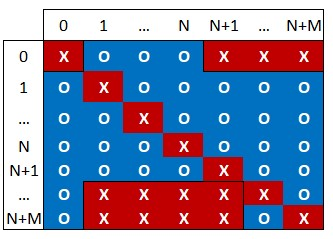
\includegraphics[scale=0.75]{Matriz factible.jpg}
\end{center}

La matriz nos muestra las variables que son instanciables desde un inicio y cuales no, debido a la naturaleza del problema (nodo consistencia). Este será el primer filtro utilizado en el proceso de instanciación, verificando en primer orden si la variable pasa por este filtro o no.


Posteriormente se da comienzo al instanciado de variables, este es realizado en etapas (las cuales también son utilizadas para el GBJ). Lo primero es clasificar las variables en secciones, de los importantes existen 6 zonas de interés:

\begin{itemize}
    \item Zona 1: Movimientos desde el depósito a clientes linehauls
    \item Zona 2: Movimientos desde clientes linehauls a clientes linehauls
    \item Zona 3: Movimientos desde clientes linehauls a clientes backhauls
    \item Zona 4: Movimientos desde clientes backhauls a clientes backhauls
    \item Zona 5: Movimientos desde clientes backhauls al depósito
    \item Zona 6: Movimientos desde clientes linehauls al depósito
\end{itemize}

\begin{center}
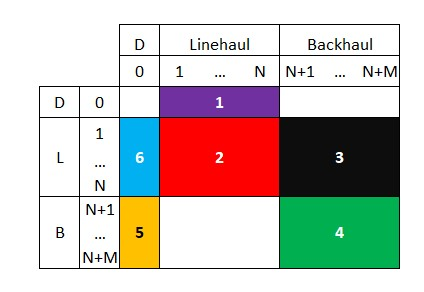
\includegraphics[scale=.75]{Fases.jpg}
\end{center}

Estas zonas son instanciadas en orden ascendente, además debido a la naturaleza binaria de las variables es posible intercambiar entre estados con facilidad, por lo tanto cuando se menciona instanciar una variable, se refiere a usarla con valor $1$, dentro de la instancia. El proceso de instanciación de las variables corresponde con cada fase, esto indica el rango del índice $i$ como $j$, el cual es constante es el rango de $k$, este siempre es recorrido entre $[0, K]$, siendo $K$ la cantidad de rutas/vehículos en la instancia del problema.

Cuando el algoritmo empieza a instanciar variables, este comienza por las zonas de manera descendente, en cada variable escogida se realiza un chequeo de factibilidad. La factibilidad que al instanciar la variable esta mantiene las restricciones del problema. Si el chequeo de factibilidad falla para la variable esta es devuelta al valor $0$ y se procede a la siguiente variable. En caso de no haber más variables en la zona actual se pasa a la siguiente zona. Cuando se pasa por todas las zonas se comprueba si la instancia obtenida es solución (dado el chequeo de factibilidad esto es siempre cierto en la primera iteración del algoritmo obteniendo una solución inicial relativamente rápida $<2$ segundos en instancias de hasta $150$ clientes y $<15$ vehículos).

Luego de una instanciación completa del problema, sea solución o no se procede a realizar el salto, este es condicionado a la cantidad de movimientos factibles realizados en cada zona. Se verifica la última zona con movimientos factibles, esta inspección es de orden descendente. Para la zona mayor con movimientos encontrada, se limpian las instanciaciones desde esa zona en orden ascendente, desde la encontrada y se utiliza una matriz de bloqueo de elementos, para no volver a seleccionar las mismas instanciaciones del ciclo que pasó recientemente y volvemos a correr el algoritmo. En el caso de encontrar una fase sin movimientos antes de encontrar una válida, limpiamos la matriz de bloqueos en esta zona y las variables instanciadas.

A forma de un ejemplo práctico de los saltos realizados, suponiendo el caso de una instanciación la cual llega al final de su ciclo. Usando las variables $M_i$ como la cantidad de movimientos factibles en la zona $i$, luego de un ciclo obtenemos los valores de movimientos $M_1=3$, $M_2=1$, $M_3=2$, $M_4=1$, $M_5=2$, $M_6=1$, esto dadas las siguientes rutas (las rutas utilizan el código de colores de la tabla de zonas anterior):

\begin{center}
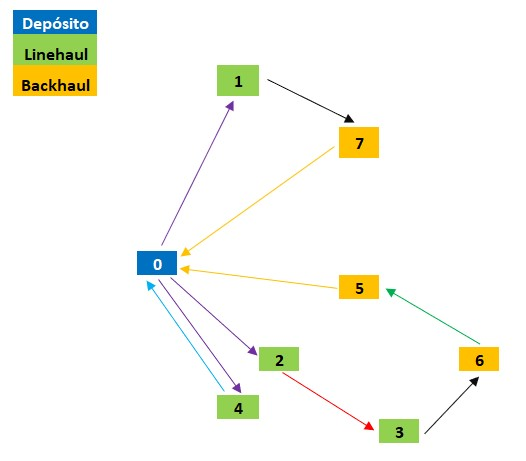
\includegraphics[scale=.5]{ruta_fases.jpg}
\end{center}

En esta situación se bloquean y eliminan las instancias de la zona 6, donde en el próximo ciclo del algoritmo se obtiene un valor de $M_6=0$, por ende se remueven los bloqueos en la zona 6 y se restablecen las instanciaciones en esa zona, la próxima zona a revisar es la zona 5, esta tiene un valor de $M_5=2$, por lo tanto se produce un comportamiento análogo al anterior, esto es debido a que estas zonas son terminales de las rutas las cuales no tiene más opciones de conexión y al bloquearlas fuerzan al algoritmo a revisar a saltar hacia atrás. Al llegar a la verificación de la zona 4 se producen eventos interesantes, primero las conexiones de la zona 6 y 5 ya no existen, además en esta zona se debe eliminar y bloquear la conexión $6 \rightarrow 5$. Al ejecutar otro ciclo del algoritmo, una nueva conexión en la zona 3 aparece al liberarse el cliente $5$, la conexión $4 \rightarrow 5$. La secuencia realizada se observa en la siguiente imagen:

\begin{center}
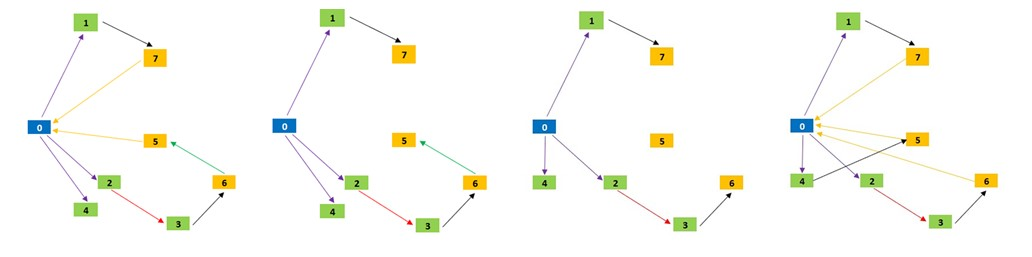
\includegraphics[scale=.45]{ruta_cambio.jpg}
\end{center}

El ciclo de funcionamiento de instanciación y saltos es cíclico, este itera hasta que se encuentra con $M_1 = 0$, una cantidad de $N + 1$ veces, siendo $N$ la cantidad de clientes tipo linehaul. Cabe destacar que al llegar al punto de $M_1 = 0$ en esa ocasión no se restablecen los bloqueos de la primera zona para permitir el uso de nuevos caminos iniciales.

\section{Experimentos}
La experimentación del algoritmo fue realizada con las instancias proporcionadas en Goestchalckx et al. (1989) \cite{goetschalckx1989vehicle}, esto debido a la variedad en la cantidad de clientes ($N+M$) como cantidad de rutas ($K$).

Dada la naturaleza del algoritmo FC, no existe cabida a la imaginación, así que los esfuerzos se centraron en las condiciones de saltos y bloqueos de las variables mencionados en la descripción del algoritmo. Al utilizar saltos dentro del algoritmo se abre la posibilidad de hacia donde saltar y cuando es adecuado hacer saltos múltiples. Así como la cantidad de bloqueos retirados en cada ciclo al encontrar movimientos no factibles dentro del algoritmo.

\subsection{Selección en el orden de las variables}
Una importante decisión dentro del algoritmo FC es el orden de instanciación de las variables. Como fue mencionado anteriormente, se produjo un despliegue por zonas. Pero aún falta definir cual es el orden de los índices dentro de cada zona.

En la sección anterior se define que las variables contienen tres índices, representando un posible arco dentro de la instancia, los índices de cada variable corresponden a el cliente de salida ($i$), el cliente de llegada ($j$) y la ruta que llevará a cabo el movimiento ($k$). Inicialmente se intentó una instanciación secuencial dentro de cada zona ($k \rightarrow i \rightarrow j$) pero el tiempo de finalización del algoritmo para instancias pequeñas era demasiado.

Finalmente, probando con diferentes instancias y órdenes de instanciación se obtuvo que los mejores resultados eran dados al invertir el orden que se intentó inicialmente. Esto tiene sentido al pensar que cada arco se prueba para cada ruta y no cada ruta prueba cada arco lo cual es más costoso de calcular (un arco tiene $k$ posibles rutas, en cuanto una ruta tiene $(N+M)^2$ posibles arcos, en donde $(N+M) > k$).

\subsection{Selección de saltos}
Dentro de la descripción del algoritmo se hace mención al método por el cual se realizan los saltos utilizados al finalizar un ciclo de instanciaciones del problema. La forma en la cual se experimentó con los saltos se debe a un intercambio de tiempo por sobre la naturaleza combinatoria del problema. 

Esto se debe que al realizar un salto de variable a variable es poco eficiente. Con lo cual se produjo cabida a la utilización del bloqueo de movimientos utilizados luego de una instanciación, lo cual crea las bifurcaciones que se crearían de forma natural en el algoritmo pero sin tener que pasar mucho tiempo dentro de estados infactibles sin encontrar soluciones. Esto genera podas del árbol en zonas las cuales podrían existir soluciones si se hubiera utilizado un carácter más greedy en cuanto a saltos.


\section{Resultados}
Como fue explicado anteriormente, las instancias utilizadas para el algoritmo son las encontradas en Goestchalckx et al. (1989) \cite{goetschalckx1989vehicle}. Para estas se consideró la cantidad de soluciones encontradas y si el algoritmo finalizó, además del tiempo de ejecución. Los datos obtenidos fueron los siguientes:

\begin{table}[H]
\begin{tabular}{|c|c|c|c|c|c|}
\hline
Instancia & N+M & K & Soluciones encontradas & Tiempo ejecucion {[}s{]} & Término del algoritmo \\ \hline
GA1 & 25  & 8 & 56  & \textless 1 & Sí \\ \hline
GA4 & 25  & 3 & 89  & \textless 1 & Sí \\ \hline
GB3 & 30  & 3 & 82  & \textless 1 & Sí \\ \hline
GF4 & 60  & 4 & 147 & $\sim$18    & Sí \\ \hline
GG2 & 57  & 6 & 194 & $\sim$36    & Sí \\ \hline
GH6 & 68  & 5 & 191 & $\sim$60    & Sí \\ \hline
GN6 & 150 & 8 & 33  & $\sim$600   & No \\ \hline
\end{tabular}
\end{table}

Se desprende de los datos que el tiempo del algoritmo es muy sensible al espacio de búsqueda de la instancia a resolver. Aún así el algoritmo es capaz de entregar una solución inicial para la instancia en menos de un segundo independiente de la cantidad de clientes o vehículos, esta característica puede ser muy útil para otros algoritmos que se basan en necesitar una solución factible inicial.

Se puede aseverar que el algoritmo cumple su cometido, pero hay espacio de mejora en cuanto al atacar instancias de mayores dimensiones, en ese caso se podría mejorar la lógica de los saltos para intentar reducir las operaciones por ciclo de instanciación del algoritmo.



\section{Conclusiones}
En este informe se presentó el estado del arte del VRPB, donde se ha descrito las perspectivas utilizadas para al resolución del problema y los resultados con estos, además de proporcionar un modelo matemático que describe el problema. Las técnicas descritas resuelven el problema, en el caso de soluciones exactas se utiliza una formulación derivada del set partitioning. Como regla general, en los métodos utilizados para resolver el problema, se hace el uso de heurísticas para obtener las soluciones, esta heurística es la cual diferencia mayoritariamente un método con los demás. El uso de una heurística por sobre otra conlleva distintos compromisos con la solución obtenida, sea la cantidad de clientes que es posible utilizar en el modelo o que tan por sobre el óptimo global estará la respuesta obtenida. Como punto adicional, cabe destacar que recientemente se han resuelto instancias relativamente grandes con tiempos de cómputo razonables, pero al crecer el tamaño del problema (visitar más clientes), se hace difícil encontrar un óptimo global dada la naturaleza del problema.

Además se experimentó utilizando una técnica de búsqueda completa (Forward Checking + Graph-Based Backjumping). En esta técnica se notó la complejidad computacional del problema, el cual al crecer la cantidad de clientes y vehículos, el tiempo necesario para obtener todas las soluciones se vuelve imposible. Se vio además la importancia de los saltos inteligentes al buscar soluciones, esto provoca un ahorro en la carga computacional del algoritmo al evitar seguir una instanciación la cual no tiene soluciones posibles. También otro punto fuerte dentro de la importancia de este algoritmo en particular es el orden de instanciación de las variables, el cual permite obtener soluciones de manera más rápida y evita instanciaciones las cuales son una pérdida de tiempo, el como también dividir las instanciaciones posibles dentro de zonas para asegurar soluciones iniciales factibles y rápidas.

VRPB tiene un interés que se mantiene vigente, más que nada por las importancia que tiene el crecimiento de la industria logística en las últimas décadas, se ha creado una importante porción de la comunidad científica a la investigación de este tipo de problemas. Una rama que no se ha explotado durante un tiempo son los algoritmos genéticos, se analizaron para resolver el problema al comienzo de la existencia de este, pero se dejo de investigar luego de aquello y el campo a obtenido sustanciales avances en los últimos años.

\newpage

\section{Bibliografía}
\bibliographystyle{plain}
\bibliography{Referencias}

\end{document} 
